\subsection{HIGHEST WEIGHT OF A FINITE DIMENSIONAL SIMPLE g-MODULE}

THEOREM 1. A simple g-module is finite dimensional if and only if it has a highest weight belonging to \(P_{++}\) .

We denote by V a simple g-module and by X its set of weights.

\begin{enumerate}
\def\labelenumi{\alph{enumi})}
\item
  Assume that V is finite dimensional. Then X is finite and non-empty (Prop. 1) and so has a maximal element \(\omega\) . Let \(\alpha \in B\) . Then \(\omega + \alpha \notin X\) , which proves that \(\omega\) is the highest weight of V (§6, no. 2, Lemma 2). On the other hand, there exists a homomorphism from \(\mathfrak{sl}(2, k)\) to g that takes H to \(H_{\alpha}\) ; by §1, Prop. 2 (i), \(\omega(H_{\alpha})\) is an integer \(\geq 0\) , so \(\omega \in P_{++}\) .
\item
  Assume that V has a highest weight \(\omega\in P_{++}\) . Let \(\alpha\in B\) and let e be a primitive element of weight \(\omega\) in V. Put \(e_{j}=X_{-\alpha}^{j}e\) for \(j\geq0\) , \(m=\omega(H_{\alpha})\in N\) , and \(N=\sum_{j=0}^{m}ke_{j}\) . By §1, no. 2, Prop. 1, \(X_{\alpha}e_{m+1}=0\) . If \(\beta\in B\) and \(\beta\neq\alpha\) , then \([X_{\beta},X_{-\alpha}]=0\) so \(X_{\beta}e_{m+1}=X_{\beta}X_{-\alpha}^{m+1}e=X_{-\alpha}^{m+1}X_{\beta}e=0\) . If \(e_{m+1}\neq0\) , we conclude that \(e_{m+1}\) is primitive, which is absurd (§6, Prop. 3 (i)); so \(e_{m+1}=0\) . Thus, by §1, no. 2, Cor. of Prop. 1, N is stable under the subalgebra \(s_{\alpha}\) generated by \(H_{\alpha},X_{\alpha}\) and \(X_{-\alpha}\) . Now \(s_{\alpha}\) is reductive in g, so the sum of the finite dimensional subspaces of V that are stable under \(s_{\alpha}\) is a g-submodule of V (Chap. I, §6, no. 6, Prop. 7); since this sum is non-zero, it is equal to V. It follows from this that \((X_{\alpha})_{V}\) and \((X_{-\alpha})_{V}\) are locally nilpotent. In view of Lemma 1 (ii), X is stable under \(s_{\alpha}\) , and this holds for all \(\alpha\) . Hence X is stable under W. Now every orbit of W on P meets \(P_{++}\) (Chap. VI, §1, no. 10). On the other hand, if \(\lambda\in X\cap P_{++}\) , then \(\lambda=\omega-\sum_{\alpha\in B}n_{\alpha}\alpha=\sum_{\alpha\in B}n'_{\alpha}\alpha\) with \(n_{\alpha}\in N\) and \(n'_{\alpha}\geq0\) for all \(\alpha\in B\) (Chap. V, §3, no. 5, Lemma 6). So \(X\cap P_{++}\) is finite and hence so is X. Since each weight has finite multiplicity (§6, no. 1, Prop. 1 (ii)), V is finite dimensional.
\end{enumerate}

COROLLARY 1. If \(\lambda \in \mathfrak{h}^*\) and \(\lambda \notin \mathrm{P}_{++}\) , the \(\mathfrak{g}\) -module \(\mathrm{E}(\lambda)\) (§6, no. 3) is infinite dimensional.

COROLLARY 2. The g-modules \(E(\lambda)\) for \(\lambda \in P_{++}\) constitute a set of representatives of the classes of finite dimensional simple g-modules.

The g-modules \(E(\lambda)\) , where \(\lambda\) is a fundamental weight, are called the fundamental g-modules; the corresponding representations are called the fundamental representations of g; they are absolutely irreducible ( \(\S6\) , no. 2, Prop. 3 (iv)).

If V is a finite dimensional g-module and \(\lambda\in P_{++}\) , the isotypical component of V of type \(\mathrm{E}(\lambda)\) is called the isotypical component of highest weight \(\lambda\) of V.

Remark 1. Let \(\lambda \in \mathrm{P}_{++}\) , \(\rho_{\lambda}\) the representation of \(\mathfrak{g}\) on \(\operatorname{E}(\lambda)\) , \(s \in \operatorname{Aut}(\mathfrak{g})\) , and \(\sigma\) the canonical image of \(s\) in \(\operatorname{Aut}(\mathrm{R},\mathrm{B})\) ( \(\S 5\) , no. 3, Cor. 1 of Prop. 5). Then \(\rho_{\lambda} \circ s\) is equivalent to \(\rho_{\sigma \lambda}\) ; indeed, if \(s \in \operatorname{Aut}_0(\mathfrak{g})\) , \(\rho_{\lambda} \circ s\) and \(\rho_{\sigma \lambda}\) are equivalent to \(\rho_{\lambda}\) (Prop. 2); and, if \(s\) leaves \(\mathfrak{h}\) and B stable, \(\rho_{\lambda} \circ s\) is simple of highest weight \(\sigma \lambda\) .

In particular, the fundamental representations are permuted by \(s\) , and this permutation is the identity if and only if \(s \in \mathrm{Aut}_0(\mathfrak{g})\) .

PROPOSITION 3. Let V be a finite dimensional g-module and X its set of weights. Let \(\lambda \in X\) , \(\alpha \in R\) , I the set of \(t \in Z\) such that \(\lambda + t\alpha \in X\) , p (resp. -q) the largest (resp. smallest) element of I. Let \(m_t\) be the multiplicity of \(\lambda + t\alpha\) .

\begin{enumerate}
\def\labelenumi{(\roman{enumi})}
\item
  I = \(\{-q, p\}\) and \(q - p = \lambda(H_{\alpha})\) .
\item
  For any integer \(u \in [0, p + q]\) , \(\lambda + (p - u)\alpha\) and \(\lambda + (-q + u)\alpha\) are conjugate under \(s_{\alpha}\) , and \(m_{-q + u} = m_{p - u}\) .
\item
  If \(t \in \mathbf{Z}\) and \(t < (p - q)/2\) , \((X_{\alpha})_{\mathrm{V}}\) maps \(V^{\lambda + t\alpha}\) injectively into \(V^{\lambda + (t + 1)\alpha}\) .
\item
  The function \(t \mapsto m_t\) is increasing on \([-q, (p - q)/2]\) and decreasing on \([(p - q)/2, p]\) .
\end{enumerate}

Let \(\alpha \in \mathrm{B}\) . Give V the \(\mathfrak{sl}(2,k)\) -module structure defined by the elements \(X_{\alpha}, X_{-\alpha}, H_{\alpha}\) of \(\mathfrak{g}\) . Every non-zero element of \(\mathrm{V}^{\lambda + p\alpha}\) is then primitive. Consequently, \((\lambda + p\alpha)(H_{\alpha}) \geq 0\) and \((X_{-\alpha})^{r}\mathrm{V}^{\lambda + p\alpha} \neq 0\) for

\[
0 \leq r \leq (\lambda + p \alpha) (H _ {\alpha}) = \lambda (H _ {\alpha}) + 2 p
\]

\pandocbounded{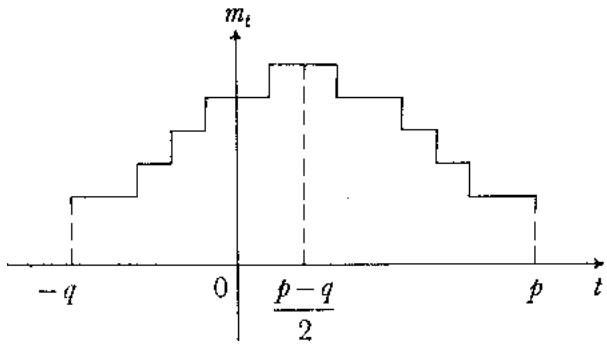
\includegraphics[keepaspectratio]{images/part001_39d2730e.jpg}}

(§1, no. 2, Prop. 2). It follows that \(\mathrm{V}^{\lambda + t\alpha} \neq 0\) for \(p \geq t \geq p - (\lambda(H_{\alpha}) + 2p)\) , so \(p + q \geq \lambda(H_{\alpha}) + 2p\) . Applying this result to \(-\alpha\) gives

\[
p + q \geq \lambda (H _ {- \alpha}) + 2 q = - \lambda (H _ {\alpha}) + 2 q.
\]

Hence \(q - p = \lambda (H_{\alpha})\) and \(\lambda + t\alpha \in \mathcal{X}\) for \(p \geq t \geq -q\) , which proves (i).

We have \(s_{\alpha}(\alpha) = -\alpha\) , and \(s_{\alpha}(\mu) \in \mu + k\alpha\) for all \(\mu \in \mathfrak{h}^*\) . Since W leaves \(\mathcal{X}\) stable (Cor. 2 of Prop. 2), \(s_{\alpha}\) leaves \(\{\lambda - q\alpha, \lambda - q\alpha + \alpha, \ldots, \lambda + p\alpha\}\) stable and takes \(\lambda - q\alpha + u\alpha\) to \(\lambda + p\alpha - u\alpha\) for all \(u \in k\) . Using Cor. 2 of Prop. 2 again, we see that \(m_{-q + u} = m_{p - u}\) for every integer \(u \in [0, p + q]\) . This proves (ii).

By §1, Cor. of Prop. 2, \((X_{\alpha})_{\mathrm{V}}|\mathrm{V}^{\lambda +t\alpha}\) is injective for \(t < (p - q) / 2\) . Now \((X_{\alpha})_{\mathrm{V}}\) maps \(\mathrm{V}^{\lambda +t\alpha}\) to \(\mathrm{V}^{\lambda +(t + 1)\alpha}\) . Hence \(m_{t + 1}\geq m_t\) for \(t < (p - q) / 2\) . Changing \(\alpha\) to \(-\alpha\) , we see that \(m_{t + 1}\leq m_t\) for \(t > (p - q) / 2\) . This proves (iii) and (iv).

COROLLARY 1. If \(\lambda \in \mathcal{X}\) and \(\lambda (H_{\alpha})\geq 1\) , then \(\lambda -\alpha \in \mathcal{X}\) . If \(\lambda +\alpha \in \mathcal{X}\) and \(\lambda (H_{\alpha}) = 0\) , then \(\lambda \in \mathcal{X}\) and \(\lambda -\alpha \in \mathcal{X}\) .

This follows immediately from Prop. 3 (i).

COROLLARY 2. Let \(\mu \in \mathrm{P}_{++}\) and \(\nu \in \mathrm{Q}_{+}\) . If \(\mu + \nu \in \mathcal{X}\) , then \(\mu \in \mathcal{X}\) .

Write \(\nu = \sum_{\alpha \in \mathrm{B}} c_{\alpha}.\alpha\) , where \(c_{\alpha} \in \mathbf{N}\) for all \(\alpha \in \mathrm{B}\) . The corollary is clear when \(\sum_{\alpha \in \mathrm{B}} c_{\alpha} = 0\) ; assume that \(\sum_{\alpha \in \mathrm{B}} c_{\alpha} > 0\) and argue by induction on \(\sum_{\alpha \in \mathrm{B}} c_{\alpha}\) . Let \((\cdot|\cdot)\) be a W-invariant non-degenerate positive symmetric bilinear form on \(\mathfrak{h}_{\mathbf{R}}^{*}\) . Then \((\nu|\sum_{\alpha \in \mathrm{B}} c_{\alpha}.\alpha) > 0\) , so there exists \(\beta \in \mathrm{B}\) such that \(c_{\beta} \geq 1\) and \((\nu|\beta) > 0\) , hence \(\nu(H_{\beta}) \geq 1\) . Since \(\mu \in \mathrm{P}_{++}\) , it follows that \((\mu + \nu)(H_{\beta}) \geq 1\) . By Cor. 1, \(\mu + (\nu - \beta) \in \mathcal{X}\) , and it suffices to apply the induction hypothesis.

COROLLARY 3. Let \(v \in V\) be primitive of weight \(\omega\) . Let \(\Sigma\) be the set of \(\alpha \in B\) such that \(\omega(H_{\alpha}) = 0\) . The stabilizer in \(\mathfrak{g}\) of the line \(kv\) is the parabolic subalgebra \(\mathfrak{p}_{\Sigma}\) associated to \(\Sigma\) (§3, no. 4, Remark).

Replacing V by the g-submodule generated by v, if necessary, we can assume that V is simple. Let s be the stabilizer. We have \((\mathfrak{n}_{+})_{\mathrm{V}}v = 0\) , \((\mathfrak{h})_{\mathrm{V}}v \subset kv\) . Let \(\alpha \in B\) be such that \(\omega(H_{\alpha}) = 0\) . We have \(\omega + \alpha \notin X\) , hence \(\omega - \alpha \notin X\) (Prop. 3 (i)) and consequently \((\mathfrak{g}^{-\alpha})_{\mathrm{V}}v = 0\) . The preceding proves that \(p_{\Sigma} \subset s\) . If \(p_{\Sigma} \neq s\) , then \(s = p_{\Sigma'}\) , where \(\Sigma'\) is a subset of B strictly containing \(\Sigma\) . Let \(\beta \in \Sigma' - \Sigma\) . Then \(g^{-\beta}\) stabilizes kv, and hence annihilates v. But, since \(\omega(H_{\beta}) > 0\) , this contradicts Prop. 3 (iii). Q.E.D.

A subset \(\mathcal{X}\) of P is called R-saturated if it satisfies the following condition: for all \(\lambda \in \mathcal{X}\) and all \(\alpha \in \mathrm{R}\) , we have \(\lambda - t\alpha \in \mathcal{X}\) for all integers \(t\) between 0 and \(\lambda(H_{\alpha})\) . Since \(s_{\alpha}(\lambda) = \lambda - \lambda(H_{\alpha})\alpha\) , we see that an R-saturated subset of P is stable under W. Let \(\mathcal{Y} \subset \mathrm{P}\) . An element \(\lambda\) of \(\mathcal{Y}\) is called R-extremal in \(\mathcal{Y}\) if, for all \(\alpha \in \mathrm{R}\) , either \(\lambda + \alpha \notin \mathcal{Y}\) or \(\lambda - \alpha \notin \mathcal{Y}\) .

PROPOSITION 4. Let \(\mathrm{V}\) be a finite dimensional \(\mathfrak{g}\) -module and \(d\) an integer \(\geq 1\) . The set of weights of \(\mathrm{V}\) of multiplicity \(\geq d\) is R-saturated.

This follows immediately from Prop. 3.

PROPOSITION 5. Let V be a finite dimensional simple g-module, \(\omega\) its highest weight, X its set of weights. Choose a W-invariant non-degenerate positive symmetric bilinear form \((\cdot|\cdot)\) on \(h_{R}^{*}\) , and let \(\lambda\mapsto\|\lambda\|=(\lambda|\lambda)^{1/2}\) be the corresponding norm.

\begin{enumerate}
\def\labelenumi{(\roman{enumi})}
\item
  \(\mathcal{X}\) is the smallest R-saturated subset of P containing \(\omega\) .
\item
  The R-extremal elements of \(\mathcal{X}\) are the W-transforms of \(\omega\) .
\item
  If \(\mu \in \mathcal{X}\) , we have \(\| \mu \| \leq \| \omega \|\) . If, in addition, \(\mu \neq \omega\) , we have \(\| \mu + \rho \| < \| \omega + \rho \|\) . If \(\mu\) is not R-extremal in \(\mathcal{X}\) , then \(\| \mu \| < \| \omega \|\) .
\item
  We have \(\mathcal{X} = \mathrm{W.}(\mathcal{X}\cap \mathrm{P}_{++})\) . An element \(\lambda\) of \(\mathrm{P}_{++}\) belongs to \(\mathcal{X}\cap \mathrm{P}_{++}\) if and only if \(\omega -\lambda \in \mathrm{Q}_{+}\) .
\item
  Let \(\mathcal{X}'\) be the smallest R-saturated subset of P containing \(\omega\) . We have \(\mathcal{X}' \subset \mathcal{X}\) (Prop. 4). Assume that \(\mathcal{X} \neq \mathcal{X}'\) . Let \(\lambda\) be a maximal element of \(\mathcal{X} - \mathcal{X}'\) . Since \(\lambda \neq \omega\) , there exists \(\alpha \in B\) such that \(\lambda + \alpha \in \mathcal{X}\) . Introduce \(p\) and \(q\) as in Prop. 3. Since \(\lambda\) is maximal in \(\mathcal{X} - \mathcal{X}'\) , \(\lambda + p\alpha \in \mathcal{X}'\) . By Prop. 3 (ii), \(\lambda - q\alpha \in \mathcal{X}'\) since \(\mathcal{X}'\) is stable under W. Hence \(\lambda + u\alpha \in \mathcal{X}'\) for every integer \(u\) in the interval \([-q, p]\) . This contradicts \(\lambda \notin \mathcal{X}'\) and proves (i).
\item
  It is clear that \(\omega\) is an R-extremal element of \(\mathcal{X}\) ; its W-transforms are therefore also R-extremal in \(\mathcal{X}\) . Let \(\lambda\) be an R-extremal element of \(\mathcal{X}\) ; we shall prove that \(\lambda \in \mathrm{W}.\omega\) . Since there exists \(w \in \mathrm{W}\) such that \(w\lambda \in \mathrm{P}_{++}\) (Chap. VI, §1, no. 10), we can assume that \(\lambda \in \mathrm{P}_{++}\) . Let \(\alpha \in \mathrm{B}\) ; introduce \(p\) and \(q\) as in Prop. 3. Since \(\lambda\) is R-extremal, either \(p = 0\) or \(q = 0\) . Since
\end{enumerate}

\[
q - p = \lambda (H _ {\alpha}) \geq 0,
\]

we cannot have \(p > 0\) . Hence \(p = 0\) and \(\lambda = \omega\) .

\begin{enumerate}
\def\labelenumi{(\roman{enumi})}
\setcounter{enumi}{2}
\tightlist
\item
  Let \(\mu \in \mathcal{X} \cap \mathrm{P}_{++}\) . Then \(\omega + \mu \in \mathrm{P}_{++}\) and \(\omega - \mu \in \mathrm{Q}_+\) (§6, no. 1, Prop. 1), so \(0 \leq (\omega - \mu|\omega + \mu) = (\omega|\omega) - (\mu|\mu)\) ; hence, \((\mu|\mu) \leq (\omega|\omega)\) , and this extends to all \(\mu \in \mathcal{X}\) by using the Weyl group. If \(\mu \in \mathcal{X} - \{\omega\}\) ,
\end{enumerate}

\[
\begin{array}{c} (\mu + \rho | \mu + \rho) = (\mu | \mu) + 2 (\mu | \rho) + (\rho | \rho) \leq (\omega | \omega) + 2 (\mu | \rho) + (\rho | \rho) \\ = (\omega + \rho | \omega + \rho) - 2 (\omega - \mu | \rho). \end{array}
\]

Now \(\omega - \mu = \sum_{\alpha \in \mathrm{B}} n_{\alpha} \alpha\) with integers \(n_{\alpha} \geq 0\) not all zero, so \((\omega - \mu | \rho) > 0\) since \((\rho | \alpha) > 0\) for all \(\alpha \in \mathrm{B}\) (Chap. VI, §1, no. 10, Prop. 29 (iii)). If \(\mu\) is not R-extremal in \(\mathcal{X}\) , there exists \(\alpha \in \mathrm{R}\) such that \(\mu + \alpha \in \mathcal{X}\) and \(\mu - \alpha \in \mathcal{X}\) ; then

\[
\| \mu \| <   \sup (\| \mu + \alpha \|, \| \mu - \alpha \|) \leq \sup _ {\lambda \in \mathcal {X}} \| \lambda \|
\]

and this last upper bound is \(\|\omega\|\) by the preceding.

\begin{enumerate}
\def\labelenumi{(\roman{enumi})}
\setcounter{enumi}{3}
\tightlist
\item
  We have \(\mathcal{X} = \mathrm{W.}(\mathcal{X}\cap \mathrm{P}_{++})\) by Chap. VI, §1, no. 10. If \(\lambda \in \mathcal{X}\) , then \(\omega -\lambda \in \mathrm{Q}_{+}\) (§6, no. 1, Prop. 1). If \(\lambda \in \mathrm{P}_{++}\) and \(\omega -\lambda \in \mathrm{Q}_{+}\) , then \(\lambda \in \mathcal{X}\) (Cor. 2 of Prop. 3).
\end{enumerate}

COROLLARY. Let X be a finite R-saturated subset of P. There exists a finite dimensional g-module whose set of weights is X.

Since \(\mathcal{X}\) is stable under W, \(\mathcal{X}\) is the smallest R-saturated set containing \(\mathcal{X} \cap \mathrm{P}_{++}\) . By Prop. 5 (i), \(\mathcal{X}\) is the set of weights of \(\bigoplus_{\lambda \in \mathcal{X} \cap \mathrm{P}_{++}} \mathrm{E}(\lambda)\) .

Remark 2. Recall (Chap. VI, §1, no. 6, Cor. 3 of Prop. 17) that there exists a unique element \(w_0\) of \(\mathrm{W}\) that transforms \(\mathrm{B}\) into \(-\mathrm{B}\) ; we have \(w_0^2 = 1\) . and \(-w_0\) respects the order relation on \(\mathrm{P}\) . With this in mind, let \(\mathrm{V}\) be a finite dimensional simple \(\mathfrak{g}\) -module, \(\omega\) its highest weight. Then \(w_0(\omega)\) is the lowest weight of \(\mathrm{V}\) , and its multiplicity is 1.

